\section{CLP LS XGK-CPUE (item 2d)}

\subsection{Organização do programa Ladder}

O CLP executa o projeto \cod{LAB\_NEW\_UPDATED}, editado no XG5000 versão 4.74 (Figuras \ref{fig:clp01} e \ref{fig:clp02}). O projeto tem dois programas de varredura e uma sub-rotina:

\begin{itemize}
    \item \textbf{BUTTONS} - trata as bordas das 12 entradas de botão \cod{P00000}-\cod{P0000B} em um único registrador de estados, \cod{D01501}, e gera as marcas internas \cod{M00020} em diante;
    \item \textbf{ANDON} - lê o relógio (\cod{DATERD}), serve a fila de comunicação com o Gateway, aplica o relógio recebido (\cod{DATEWRP}), executa as máquinas de estados dos 12 postos e gera o comando do motor;
    \item \textbf{MENSAGEM\_ANDON} - sub-rotina que grava cada evento, em oito palavras, na FIFO \cod{D00300} com \cod{FIWR}.
\end{itemize}

\begin{figure}[H]
    \centering
    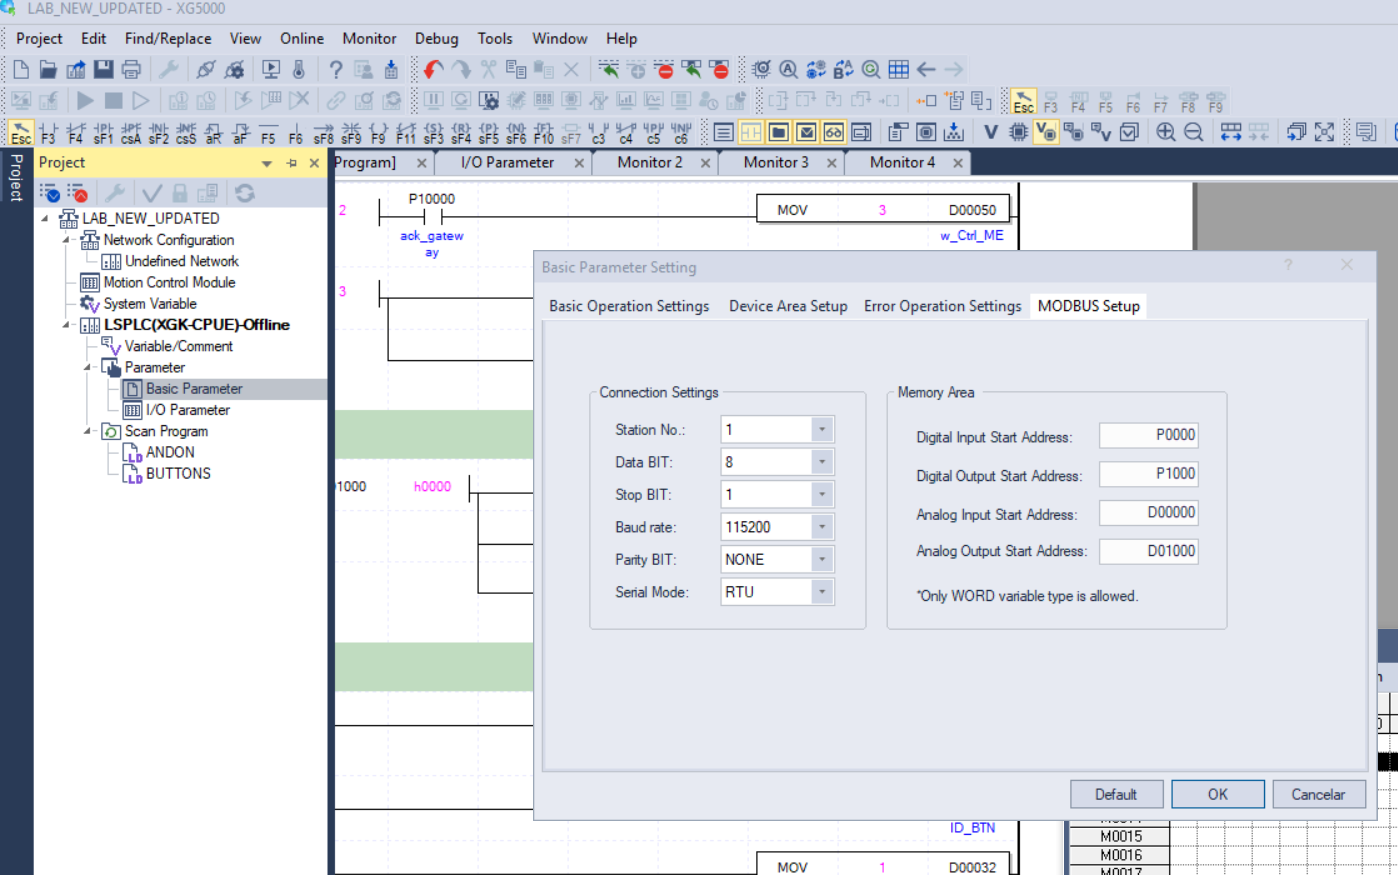
\includegraphics[width=0.80\textwidth]{Imagens/clp_01_configuracao_modbus.png}
    \caption{XG5000, \textit{Basic Parameter} $\rightarrow$ \textit{MODBUS Setup}: estação 1, 115200 baud, 8 bits, sem paridade, 1 bit de parada, modo RTU; áreas \cod{P0000}, \cod{P1000}, \cod{D00000} e \cod{D01000}. (arquivo: Imagens/clp\_01\_configuracao\_modbus.png)}
    \label{fig:clp01}
\end{figure}

\begin{figure}[H]
    \centering
    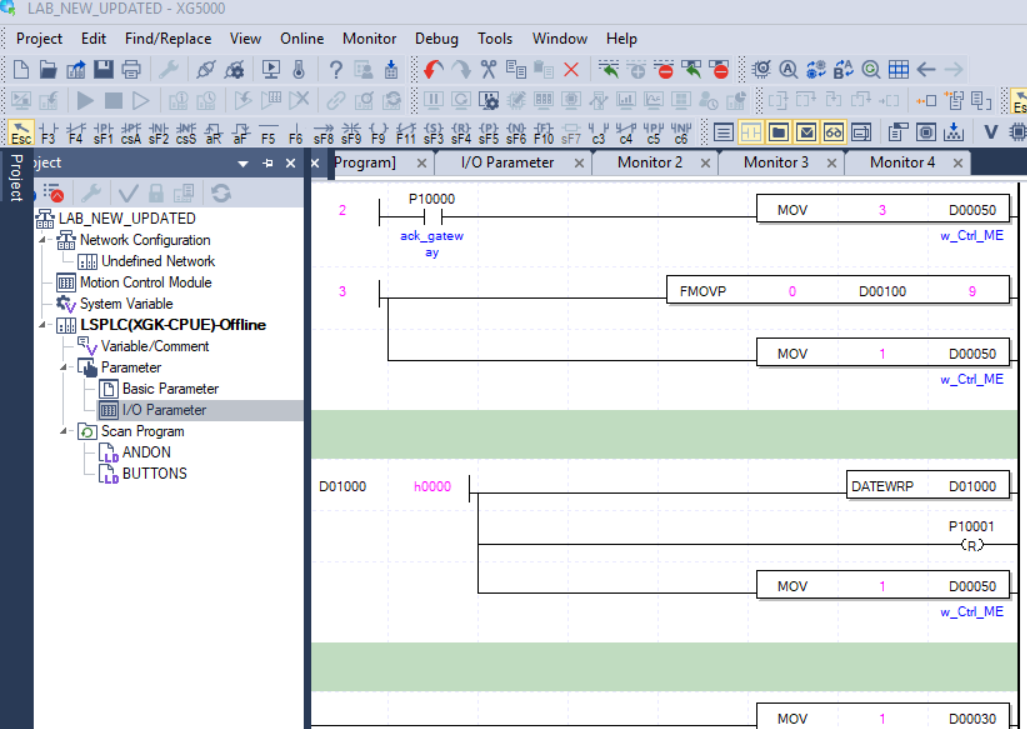
\includegraphics[width=0.62\textwidth]{Imagens/clp_02_arvore_projeto.png}
    \caption{Árvore do projeto \cod{LAB\_NEW\_UPDATED} com a CPU XGK-CPUE e os programas ANDON e BUTTONS em \textit{Scan Program}. (arquivo: Imagens/clp\_02\_arvore\_projeto.png)}
    \label{fig:clp02}
\end{figure}

\subsection{Mapa Modbus}

O Gateway é o cliente Modbus RTU e o CLP é o servidor. A Tabela \ref{tab:mapa} é o mapa efetivamente configurado em \cod{hardware/deploy/config.raspberry.toml}. O endereço Modbus tem base zero dentro de cada área; a área de \textit{Holding Registers} começa em \cod{D01000} e a de \textit{Input Registers} em \cod{D00000}, por isso \cod{D16052} corresponde ao \textit{holding register} 15052.

{\footnotesize
\begin{longtable}{|>{\raggedright\arraybackslash}p{2.6cm}|>{\raggedright\arraybackslash}p{2.9cm}|>{\centering\arraybackslash}p{1.9cm}|>{\raggedright\arraybackslash}p{7.2cm}|}
\caption{Mapa Modbus entre o Gateway e o CLP.}\label{tab:mapa}\\
\hline
\textbf{XG5000} & \textbf{Área / função} & \textbf{Endereço} & \textbf{Conteúdo} \\ \hline
\endfirsthead
\hline
\textbf{XG5000} & \textbf{Área / função} & \textbf{Endereço} & \textbf{Conteúdo} \\ \hline
\endhead
\cod{D00100} & Input Reg., FC04 & 100 & Palavras pendentes na fila (0, 8, 16...). \\ \hline
\cod{D00101}-\cod{D00108} & Input Reg., FC04 & 101-108 & Evento de 16 bytes; \cod{D00101 = 1}. \\ \hline
\cod{D00109}-\cod{D00111} & Input Reg., FC04 & 109-111 & Estado instantâneo dos Andons, 4 postos por palavra, 1 bit por categoria. \\ \hline
\cod{D00112} & Input Reg., FC04 & 112 & Comando do motor: 1 ligado, 0 desligado. \\ \hline
\cod{D00113}-\cod{D00160} & Input Reg., FC04 & 113-160 & Por posto, Takt time e último ciclo em UInt32 (palavra baixa primeiro, décimos de segundo). \\ \hline
\cod{D01000}-\cod{D01003} & Holding Reg., FC16 & 0-3 & Relógio em BCD para \cod{DATEWRP}. \\ \hline
\cod{D01200} & Holding Reg., FC03/FC06 & 200 & Velocidade do motor, 0 a 100 \%. \\ \hline
\cod{D01201.0} & Holding Reg., FC03/FC06 & 201, bit 0 & Pedido de parada da linha. \\ \hline
\cod{D01651}-\cod{D01662} & Holding Reg., FC03 & 651-662 & Estado dos postos P01 a P12 (0 a 3). \\ \hline
\cod{D16052} & Holding Reg., FC03 & 15052 & Contador de produção (peças concluídas no P12). \\ \hline
\cod{D17001}-\cod{D17288} & Holding Reg., FC16/FC03 & 16001-16288 & Base de tempos: 24 palavras por posto. \\ \hline
\cod{P10000} & Coil, FC05 & 0 & ACK do evento lido pelo Gateway. \\ \hline
\cod{P10001} & Coil, FC05 & 1 & Pedido de aplicação do relógio. \\ \hline
\cod{P10002} & Coil, FC05 & 2 & Pulso de Start (2 s). \\ \hline
\cod{P10003} & Coil, FC05 & 3 & Pulso de reset dos postos (2 s). \\ \hline
\end{longtable}
}

\subsection{Botões e geração dos eventos de Andon}

O programa BUTTONS usa um único registrador para as 12 entradas. \cod{D01501} parte de 100 e, para a entrada de posição \textit{n} (1 a 12), percorre \cod{100} $\rightarrow$ \textit{n} (borda de descida) $\rightarrow$ \textit{n}+12 (subida) $\rightarrow$ \textit{n}+24 (descida) $\rightarrow$ \cod{100} (subida). Os três estados intermediários mantêm ativa a marca do botão (para \cod{P00000}, \cod{M00020} ativa em 1, 13 e 25). Cada borda da marca dispara, no programa ANDON, o preenchimento de posto (\cod{D00030}), botão (\cod{D00031}) e estado (\cod{D00032}: 1 ligado, 2 desligado) e chama \cod{MENSAGEM\_ANDON}, que enfileira tipo, posto, data e hora (lidos por \cod{DATERD} em \cod{D00040}-\cod{D00043}), botão e estado (Figura \ref{fig:clp13}).

A entrega ao Gateway é controlada por \cod{D00050} (Figuras \ref{fig:clp09} e \ref{fig:clp10}): em \textbf{1}, se a FIFO não está vazia, o Ladder copia o cabeçalho para \cod{D00100} e retira as oito palavras para \cod{D00101}-\cod{D00108} com \cod{FIFRDP}; em \textbf{2}, mantém o evento disponível até o Gateway ligar \cod{P10000}; em \textbf{3}, zera as nove palavras com \cod{FMOVP} e volta a 1.

\begin{figure}[H]
    \centering
    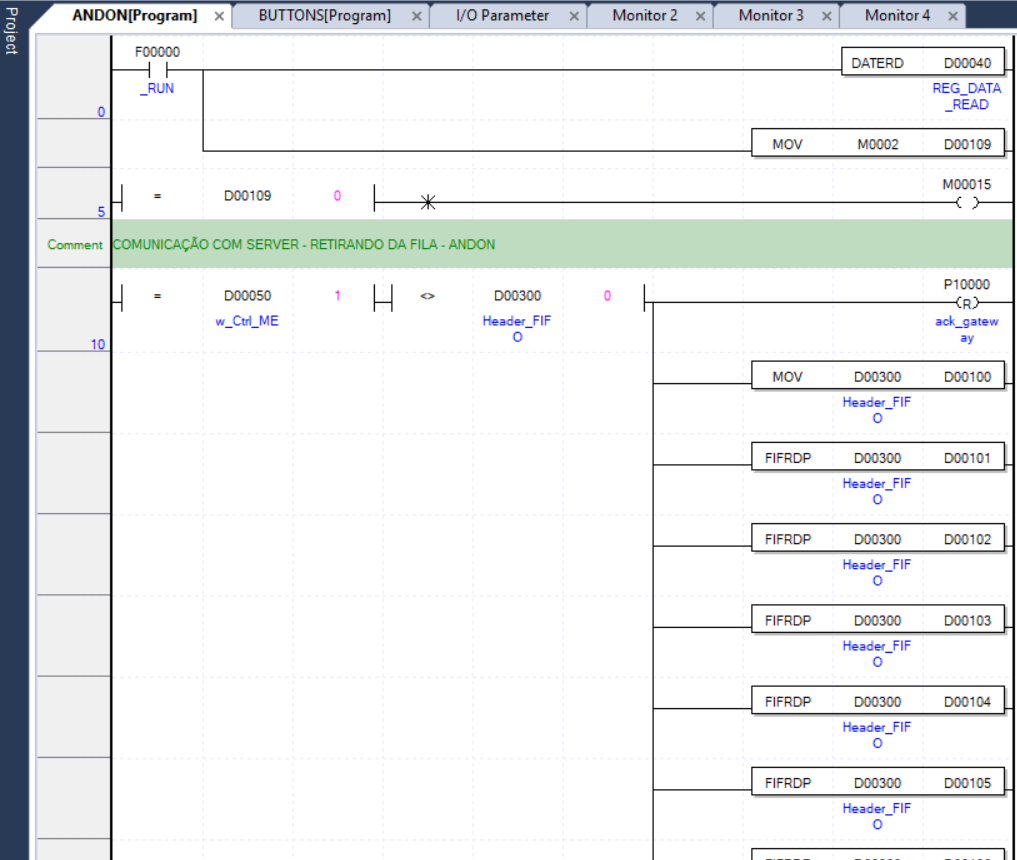
\includegraphics[width=0.78\textwidth]{Imagens/clp_09_andon_leitura_fila.png}
    \caption{Programa ANDON: \cod{DATERD} em \cod{D00040} e início da retirada da FIFO \cod{D00300} para \cod{D00100}-\cod{D00108} quando \cod{D00050 = 1}. (arquivo: Imagens/clp\_09\_andon\_leitura\_fila.png)}
    \label{fig:clp09}
\end{figure}

\begin{figure}[H]
    \centering
    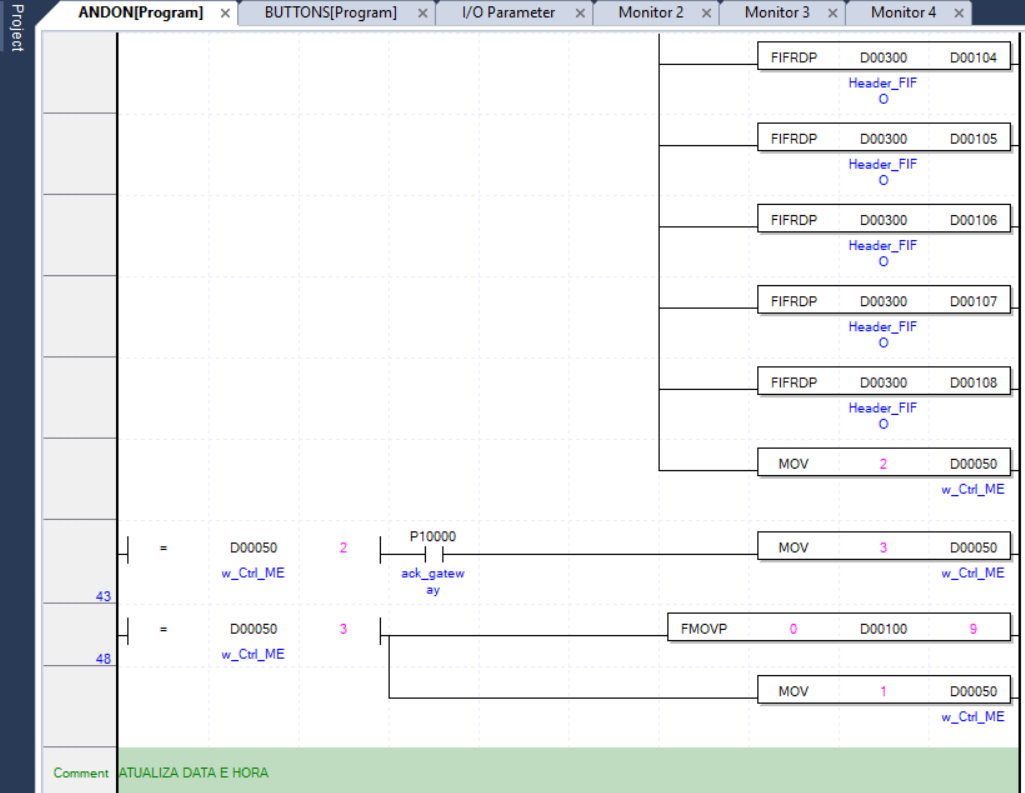
\includegraphics[width=0.78\textwidth]{Imagens/clp_10_andon_ack_gateway.png}
    \caption{Fim da retirada (\cod{MOV 2 D00050}), espera do ACK \cod{P10000} (\cod{MOV 3 D00050}) e limpeza do bloco com \cod{FMOVP 0 D00100 9}. (arquivo: Imagens/clp\_10\_andon\_ack\_gateway.png)}
    \label{fig:clp10}
\end{figure}

\begin{figure}[H]
    \centering
    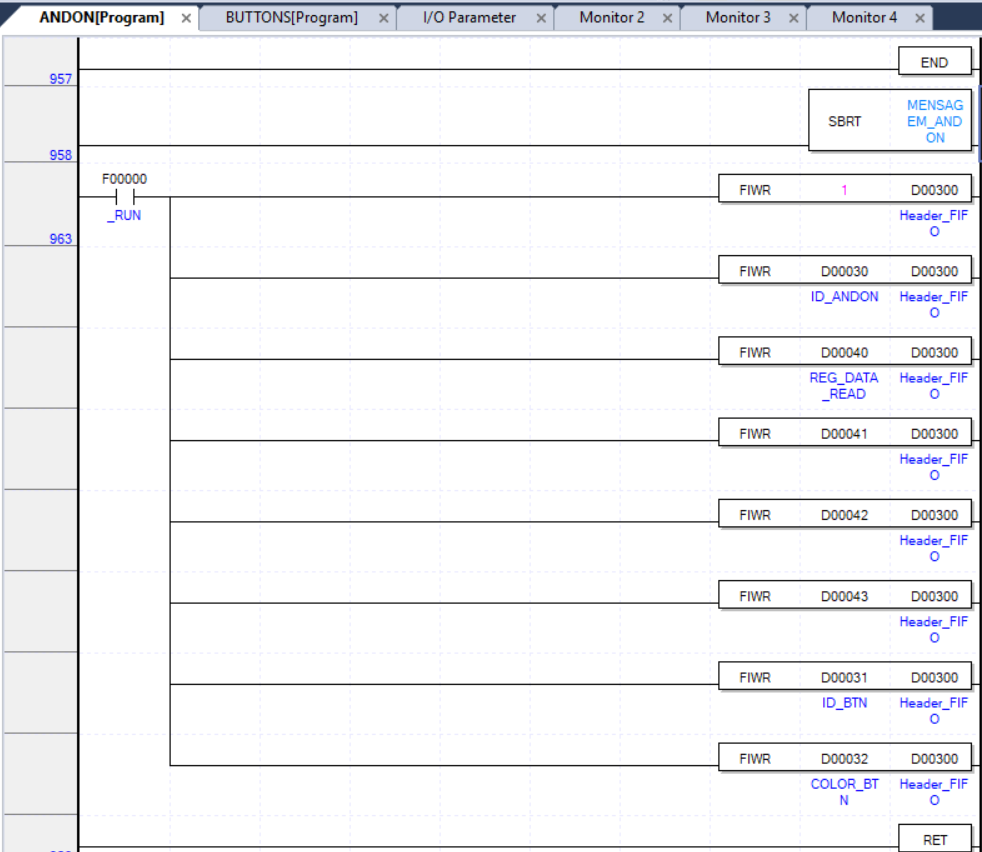
\includegraphics[width=0.78\textwidth]{Imagens/clp_13_andon_gravacao_fila.png}
    \caption{Sub-rotina \cod{MENSAGEM\_ANDON}: sete \cod{FIWR} gravam na FIFO \cod{D00300} o tipo, o posto, as quatro palavras de data e hora, o botão e o estado. (arquivo: Imagens/clp\_13\_andon\_gravacao\_fila.png)}
    \label{fig:clp13}
\end{figure}

\subsection{Máquinas de estados dos postos}

Cada posto tem uma palavra de estado (\cod{D01651} a \cod{D01662}): \textbf{0} espera, \textbf{1} preparação, \textbf{2} medição (processando) e \textbf{3} fim do ciclo. Nos postos 01 e 02, a passagem 2 $\rightarrow$ 3 ocorre no fim do temporizador cujo \textit{preset} é o tempo da base (\cod{D17001[Z001]}, \cod{D17025[Z002]}); no P07, manual, ocorre na borda de \cod{P0000D}. Os postos automáticos 08 a 10 vão direto de 0 para 2 quando o sensor de entrada confirma a peça e encerram a medição na borda do sensor seguinte. Na passagem 3 $\rightarrow$ 0 o Ladder copia o tempo medido para o bloco de telemetria (\cod{D00115}, \cod{D00119}, ..., \cod{D00151}), incrementa o contador do posto (\cod{D16041}-\cod{D16050}) e habilita o posto seguinte. A borda de \cod{P10002} ativa \cod{M00101}, entrada do P01 (Start); \cod{P10003} zera estados, temporizadores e contadores (reset). O motor é ligado (\cod{D00112.0}) quando \cod{D01501 = 100}, isto é, nenhum Andon pressionado, e algum dos postos 08 a 10 está em estado diferente de 0 (Figuras \ref{fig:clp15}, \ref{fig:clp17} e \ref{fig:clp21}).

\begin{figure}[H]
    \centering
    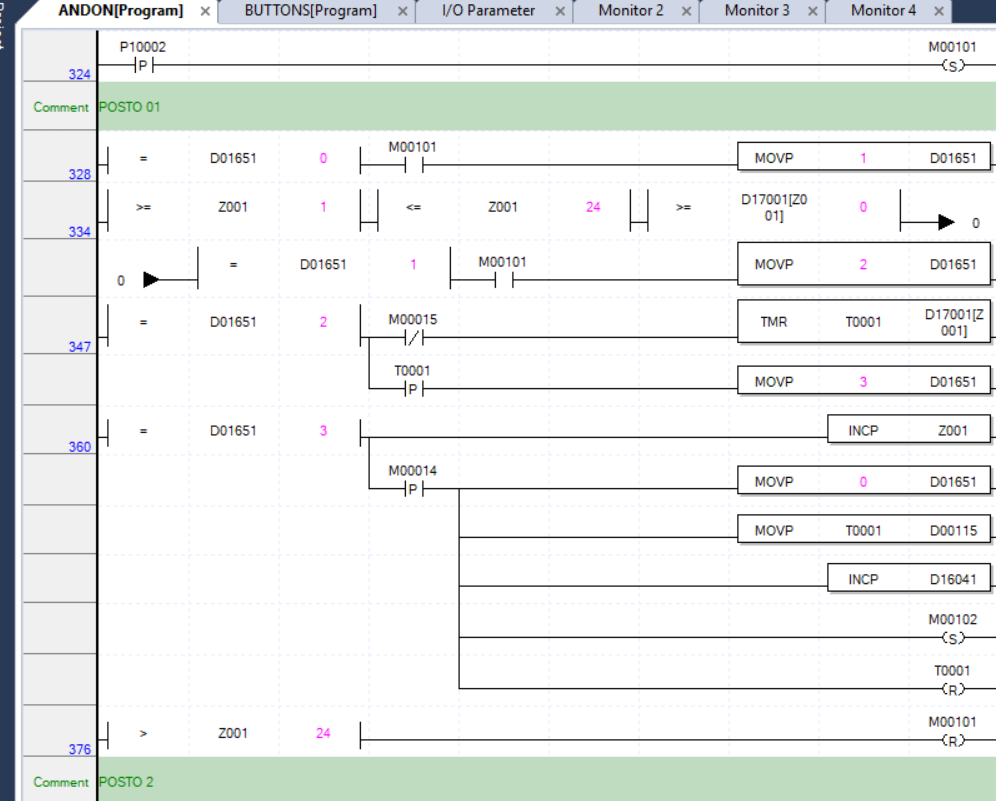
\includegraphics[width=0.78\textwidth]{Imagens/clp_15_posto_01.png}
    \caption{Posto 01: estado em \cod{D01651}, temporizador \cod{T0001} com \textit{preset} indexado \cod{D17001[Z001]}, cópia do tempo para \cod{D00115} e incremento de \cod{D16041}. (arquivo: Imagens/clp\_15\_posto\_01.png)}
    \label{fig:clp15}
\end{figure}

\begin{figure}[H]
    \centering
    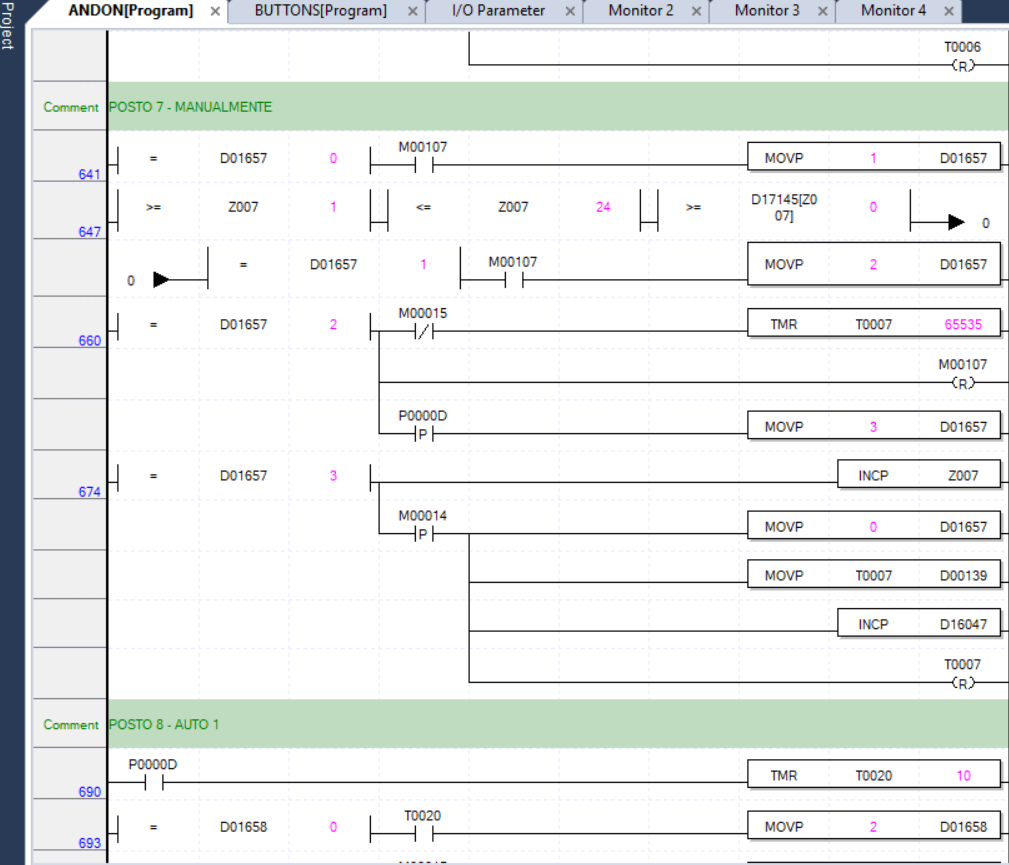
\includegraphics[width=0.78\textwidth]{Imagens/clp_17_posto_07_manual.png}
    \caption{Posto 07 (manual): estado em \cod{D01657}; a borda de \cod{P0000D} leva ao estado 3. É a transição 1 $\rightarrow$ 2 deste posto que sincroniza a IT Digital E07 (seção 7). (arquivo: Imagens/clp\_17\_posto\_07\_manual.png)}
    \label{fig:clp17}
\end{figure}

\begin{figure}[H]
    \centering
    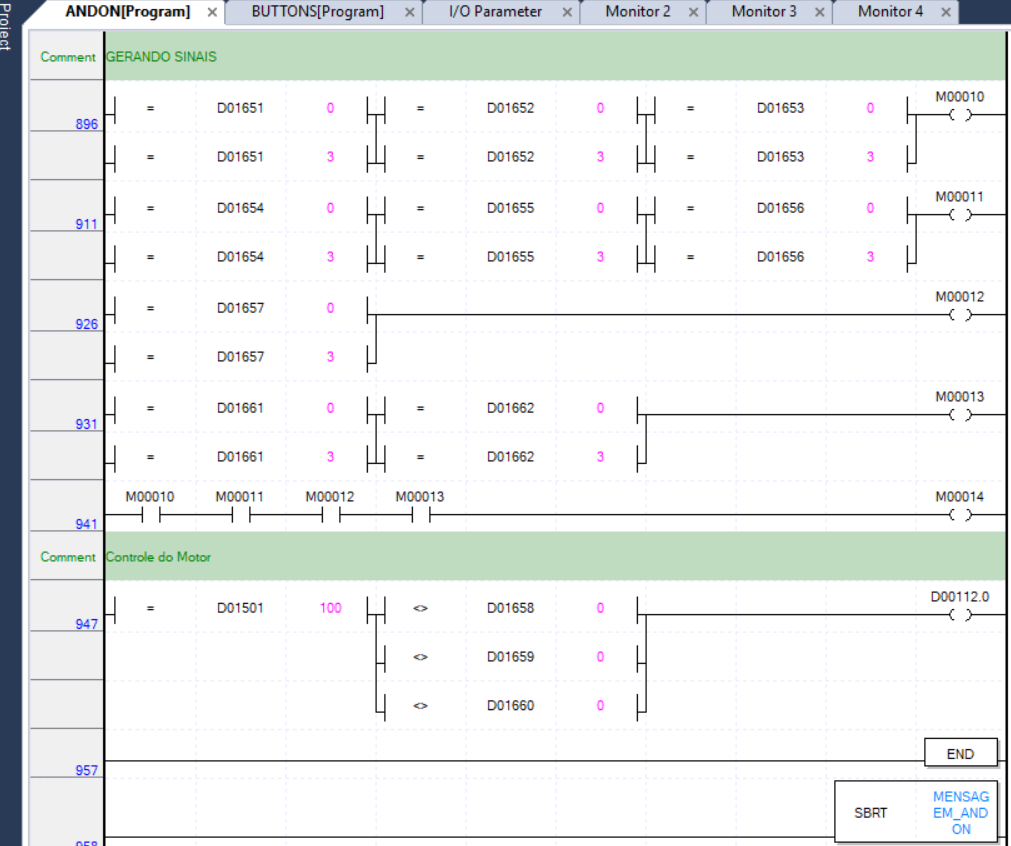
\includegraphics[width=0.78\textwidth]{Imagens/clp_21_sinais_e_motor.png}
    \caption{Geração de \cod{M00014} a partir de \cod{M00010}-\cod{M00013} e condição da saída \cod{D00112.0} (comando do motor). (arquivo: Imagens/clp\_21\_sinais\_e\_motor.png)}
    \label{fig:clp21}
\end{figure}

As demais 13 capturas do XG5000 estão no Anexo (Figuras A1 a A13).

\subsection{Evidência: eventos reais lidos do CLP}

Em 27/09/2026 o Gateway \cod{LINHA\_A} foi executado com o CLP real ligado à porta COM10 por um adaptador USB-RS232. O banco \cod{hardware/data/gateway.db} registra 18 eventos de Andon, todos do posto P05 (o botão cabeado na bancada): 6 de Processo, 6 de Equipamento, 4 de Qualidade e 2 de Material, sempre em pares ligado/desligado. A Tabela \ref{tab:decode} decodifica, byte a byte, o primeiro evento tal como o CLP o publicou em \cod{D00101}-\cod{D00108}.

{\footnotesize
\begin{longtable}{|>{\centering\arraybackslash}p{1.4cm}|>{\centering\arraybackslash}p{1.9cm}|>{\raggedright\arraybackslash}p{3.4cm}|>{\raggedright\arraybackslash}p{7.6cm}|}
\caption{Decodificação do evento 1 de \cod{gateway.db} (\cod{event\_uid} \cod{LINHA\_A-20260927165903-3DE06210}). Bytes em hexadecimal: \cod{00 01 00 05 09 26 16 27 03 59 20 00 00 03 00 01}.}\label{tab:decode}\\
\hline
\textbf{Bytes} & \textbf{Valor (hex)} & \textbf{Campo} & \textbf{Interpretação} \\ \hline
\endfirsthead
\hline
\textbf{Bytes} & \textbf{Valor (hex)} & \textbf{Campo} & \textbf{Interpretação} \\ \hline
\endhead
0-1 & \cod{00 01} & Tipo & 1 = evento de Andon gerado pelo CLP (\cod{D00101}). \\ \hline
2-3 & \cod{00 05} & Posto & P05. \\ \hline
4 / 5 & \cod{09} / \cod{26} & Mês / ano (BCD) & Setembro de (20)26. \\ \hline
6 / 7 & \cod{16} / \cod{27} & Hora / dia (BCD) & 16 h, dia 27. \\ \hline
8 / 9 & \cod{03} / \cod{59} & Segundo / minuto (BCD) & 59 min 03 s. \\ \hline
10 / 11 & \cod{20} / \cod{00} & Século / dia da semana & Século 20; dia da semana 0 = domingo (27/09/2026 foi domingo). \\ \hline
12-13 & \cod{00 03} & Botão & 3 = Processo (Andon verde). \\ \hline
14-15 & \cod{00 01} & Estado & 1 = ligado. \\ \hline
\end{longtable}
}

O resultado, ``P05, Processo, ligado, 27/09/2026 16:59:03'', coincide com as colunas \cod{station}, \cod{button\_id}, \cod{status} e \cod{occurred\_at} gravadas pelo Gateway e com a linha correspondente do receptor (\cod{reception}, primeira recepção, às 16:59:04,04). O identificador do evento combina o Gateway, o carimbo de tempo do pacote e o CRC32 dos 16 bytes. A lista completa dos 18 eventos está na Tabela A1 do Anexo.

A Figura \ref{fig:latencia} mostra, para cada evento, o tempo entre a gravação no SQLite e o ACK \cod{P10000} escrito no CLP e, em seguida, até o ACK TCP do receptor. O ACK no CLP levou entre 13,4 e 17,3 ms (mediana 15,9 ms) e a entrega completa, entre 23,4 e 39,9 ms (mediana 33,9 ms). Nenhum evento precisou de nova tentativa (\cod{attempts = 0}).

\begin{figure}[H]
    \centering
    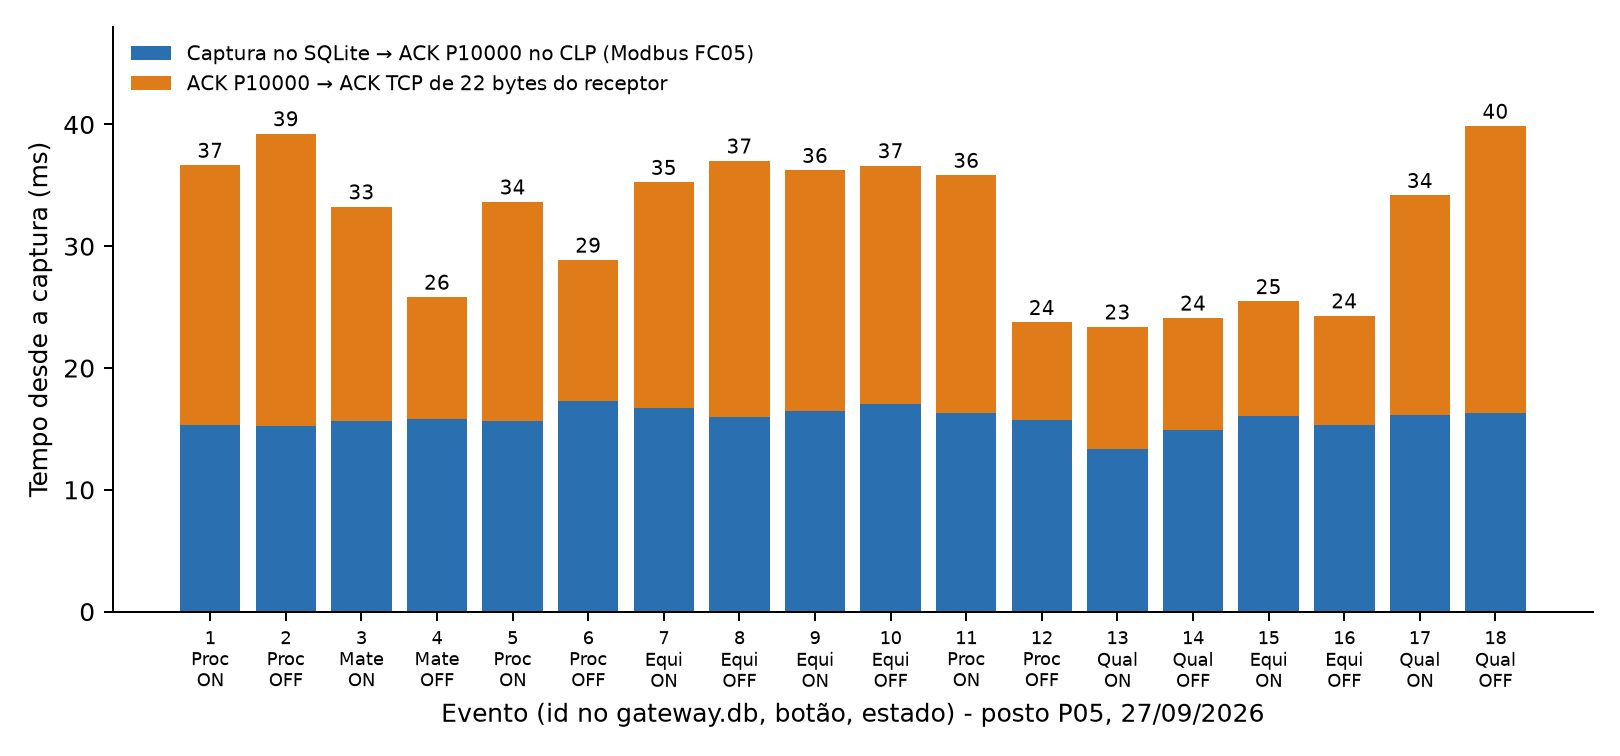
\includegraphics[width=1.00\textwidth]{Imagens/ev_latencia_eventos_reais.png}
    \caption{Latência dos 18 eventos reais (CLP LS XGK, 27/09/2026), calculada a partir de \cod{captured\_at}, \cod{plc\_acknowledged\_at} e \cod{confirmed\_at} de \cod{gateway.db}. (arquivo: Imagens/ev\_latencia\_eventos\_reais.png)}
    \label{fig:latencia}
\end{figure}

\textbf{Retenção na FIFO durante a perda de comunicação.} Às 20:48:23 o Gateway deixou de receber respostas do CLP e, em seguida, a porta COM10 desapareceu (adaptador desconectado). Os eventos 13 a 16 têm carimbo do CLP entre 22:19:09 e 22:19:56, ou seja, foram gerados enquanto o Gateway estava sem comunicação. Eles ficaram retidos na FIFO \cod{D00300} e foram capturados na reconexão, às 22:26:21,69, 22:26:21,91, 22:26:22,17 e 22:26:22,42 - um evento a cada ciclo de leitura de 250 ms, na ordem original e sem perda. A regra ``um evento por vez, liberado somente após \cod{P10000}'' do Ladder é o que garante esse comportamento.
